\chapter{Trigonometric Ratios of Any Angle and Sign}
\section{Angle of $45^\circ$}
\begin{center}
  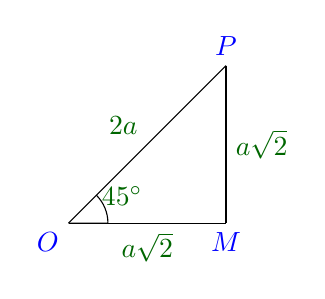
\begin{tikzpicture}
    \draw (0, 0) -- (2, 0);
    \draw (0, 0) -- (2, 2);
    \draw (2, 2) -- (2, 0);
    \draw [blue] (0,0) node[anchor=north east] {$O$};
    \draw [blue] (2,0) node[anchor=north] {$M$};
    \draw [blue] (2,2) node[anchor=south] {$P$};
    \draw (0, 0) -- (0.5, 0) arc[start angle=0, end angle=45, radius=0.5];
    \draw [black!60!green] (0.3, 0.1) node[anchor=south west] {$45^\circ$} ;
    \draw [black!60!green] (1, 0) node[anchor=north] {$a\sqrt{2}$};
    \draw [black!60!green] (2, 1) node[anchor=west] {$a\sqrt{2}$};
    \draw [black!60!green] (1, 1) node[anchor=south east] {$2a$};
  \end{tikzpicture}
\end{center}

Consider the above figure, which is a right-angle triangle, drawn so that $\angle OMP=90^\circ$ and $\angle MOP=45^\circ$. We know
that the sum of all angles of a triangle is $180^\circ$. Thus,

$$\angle OPM = 180^\circ - \angle MOP - \angle OMP = 180^\circ - 90^\circ - 45^\circ = 45^\circ$$

$\therefore OM = MP$. Let $OP=2a,$ then from Pythagora theorem, we can write

$$4a^2 = OP^2 = OM^2 + MP^2 = 2OM^2 \Rightarrow Om = a\sqrt{2} = MP$$

$\sin45^\circ = \frac{MP}{OP} = \frac{a\sqrt{2}}{2a} = \frac{1}{\sqrt{2}}$.

Other trigonometric ratios can be deduced similarly for this angle.

\section{Angles of $30^\circ$ and $60^\circ$}
\begin{center}
  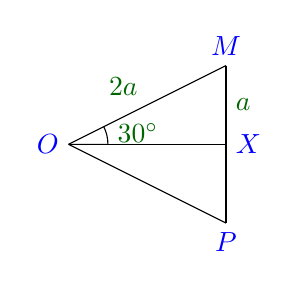
\begin{tikzpicture}
    \draw (0, 0) -- (2, 0);
    \draw (2, -1) -- (2, 1);
    \draw (0, 0) -- (2, 1);
    \draw (0, 0) -- (2, -1);
    \draw [blue] (0, 0) node[anchor=east] {$O$};
    \draw [blue] (2, 1) node[anchor=south] {$M$};
    \draw [blue] (2, -1) node[anchor=north] {$P$};
    \draw (0, 0) -- (0.5, 0) arc[start angle=0, end angle=27, radius=0.5];
    \draw [black!60!green] (0.5, -.1) node[anchor=south west] {$30^\circ$} ;
    \draw [black!60!green] (2, 0.5) node[anchor=west] {$a$};
    \draw [black!60!green] (1, 0.5) node[anchor=south east] {$2a$};
    \draw [blue] (2, 0) node[anchor=west] {$X$};
  \end{tikzpicture}
\end{center}
Consider an equilateral $\triangle OMP$. Let the sides $OM, OP, MP$ be each $2a$. We draw a bisector of $\angle MOP$, which will be
a perpendicular bisector of $MP$ at $X$ because the triangle is equilateral. Thus, $MX = a$. In $\triangle OMX, OM=2a, \angle
MOX=30^\circ, \angle OXM=90^\circ$ because each angle in an equilateral triangle is $60^\circ$.

$\sin MOX=\frac{MX}{OM} = \frac{1}{2}\Rightarrow \sin30^\circ = \frac{1}{2}$

Similarly, $\angle OMX=60^\circ$ because the sum of all angles of a triangle is $180^\circ$.

$\cos OMX = \frac{MX}{OM} = \frac{1}{2}\Rightarrow \cos60^\circ = \frac{1}{2}$

All other trigonometric ratios can be found from these two.

\section{Angle of $0^\circ$}
\begin{center}
  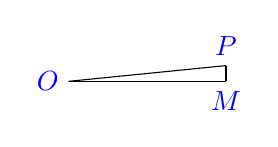
\begin{tikzpicture}
    \draw (0, 0) -- (2, 0);
    \draw (0, 0) -- (2, .2);
    \draw (2, 0) -- (2, .2);
    \draw [blue] (0, 0) node[anchor=east] {$O$};
    \draw [blue] (2, 0) node[anchor=north] {$M$};
    \draw [blue] (2, .2) node[anchor=south] {$P$};
  \end{tikzpicture}
\end{center}


Consider the $\triangle MOP$ such that side $MP$ is smaller than any quantity we can assign i.e. what we denote by $0$. Thus,
$\angle MOP$ is what is called approaching $0$ or $\lim_{x\to 0}$ in terms of calculus. Why we take such a value is because if any
angle of a triangle is equal to $0^\circ$ then the triangle won't exist. Thus these values are limiting values as you will learn in
calculus.

However, in this case, $\sin0^\circ = \dfrac{MP}{OP} = \frac{0}{OP} = 0$. Other trigonometric ratios can be found from this easily.

\section{Angle of $90^\circ$}
In the previous figure, as $\angle OMP$ will approach $0^\circ$, the $\angle OPM$ will approach $90^\circ$. Also, $OP$ will
approach the length of $OM$. Similar to previous case, in right-angle trianglee if one angle (other than right angle) approaches
$0^\circ$ the other one will appraoch $90^\circ$ and at that value the triangle will cease to exist.

Thus, $\sin90^\circ = \dfrac{OM}{OP} = \frac{OP}{OP} = 1$. Now other angles can be found easily from this.

Given below is a table of most useful angles:

\begin{longtable}{|l|l|l|l|l|l|}
  \hline
  \textbf{Angle} & $0^\circ$ & $30^\circ$ & $45^\circ$ & $60^\circ$ & $90^\circ$\\
  \hline
  $\sin$ & $0$ & $\frac{1}{2}$ & $\frac{1}{\sqrt{2}}$ & $\frac{\sqrt{3}}{2}$ & $1$\\
  \hline
  $\cos$ & $1$ & $\frac{\sqrt{3}}{2}$ & $\frac{1}{\sqrt{2}}$ & $\frac{1}{2}$ & $0$\\
  \hline
  $\tan$ & $0$ & $\frac{1}{\sqrt{3}}$ & $1$ & $\sqrt{3}$ & $\infty$\\
  \hline
  $\cot$ & $\infty$ & $\sqrt{3}$ & $1$ & $\frac{1}{\sqrt{3}}$ & $0$\\
  \hline
  $\sec$ & $1$ & $\frac{2}{\sqrt{3}}$ & $\sqrt{2}$ & $2$ & $\infty$\\
  \hline
  cosec & $\infty$ & $2$ & $\sqrt{2}$ & $\frac{2}{\sqrt{3}}$ & $1$\\
  \hline
\end{longtable}
\section{Complementary Angles}
\begin{center}
  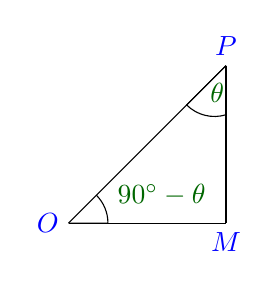
\begin{tikzpicture}
    \draw (0, 0) -- (2, 0);
    \draw (0, 0) -- (2, 2);
    \draw (2, 0) -- (2, 2);
    \draw [blue] (0, 0) node[anchor=east] {$O$};
    \draw [blue] (2, 0) node[anchor=north] {$M$};
    \draw [blue] (2, 2) node[anchor=south] {$P$};
    \draw (0, 0) -- (0.5, 0) arc[start angle=0, end angle=45, radius=0.5];
    \draw (2, 2) -- (1.5, 1.5) arc[start angle=225, end angle=287, radius=0.5];
    \draw [black!60!green] (0.5, .1) node[anchor=south west] {$90^\circ - \theta$} ;
    \draw [black!60!green] (2.1, 1.9) node[anchor=north east] {$\theta$};
  \end{tikzpicture}
\end{center}

Angles are said to be complementary if their sum is equal to one right angle i.e. $90^\circ$. Thus, if measure of one angle is
$\theta$ the other will automatically be $90^\circ - \theta$.

Consider the figure. $\triangle OMP$ is a right-angle triangle, whose $\angle OMP$ is a right angle. Since the sum of all angles is
$180^\circ$, therefore sum of $\angle MOP$ and $\angle MPO$ will be equalto one right angle or $90^\circ$ i.e. they are
complementary angles.

Let $\angle MPO = \theta$ then $\angle MOP = 90^\circ - \theta$. When $\angle MPO$ is considered $MP$ becomes the base and $OM$
becomes the perpendicular.

Thus, $\sin(90^\circ - \theta) = \sin MOP = \frac{MP}{OP} = \cos MPO = \cos\theta$

$\cos(90^\circ - \theta) = \sin MPO = \frac{MO}{OP} = \sin\theta$

$\tan(90^\circ - \theta) = \tan MOP = \frac{PM}{OM} = \cot MPO = \cot\theta$

Similarly, $\cot(90^\circ - \theta) =\tan\theta, {\rm cosec}(90^\circ - \theta) = \sec\theta, \sec(90^\circ - \theta) = {\rm
cosec}\theta$.

\section{Supplementary Angles}
\begin{center}
  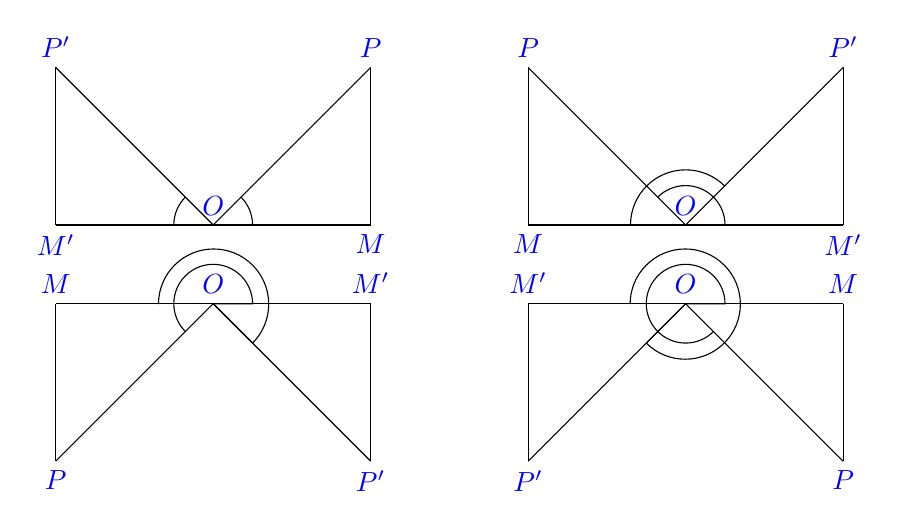
\begin{tikzpicture}
    \draw (0, 0) -- (2, 0);
    \draw (0, 0) -- (2, 2);
    \draw (2, 0) -- (2, 2);
    \draw [blue] (0, 0) node[anchor=south] {$O$};
    \draw [blue] (2, 0) node[anchor=north] {$M$};
    \draw [blue] (2, 2) node[anchor=south] {$P$};
    \draw (0, 0) -- (0.5, 0) arc[start angle=0, end angle=45, radius=0.5];
    \draw (0, 0) -- (-2, 0);
    \draw (0, 0) -- (-2, 2);
    \draw (-2, 0) -- (-2, 2);
    \draw [blue] (-2, 0) node[anchor=north] {$M'$};
    \draw [blue] (-2, 2) node[anchor=south] {$P'$};
    \draw (0, 0) -- (-0.5, 0) arc[start angle=180, end angle=135, radius=0.5];

    \draw (6, 0) -- (8, 0);
    \draw (6, 0) -- (8, 2);
    \draw (8, 0) -- (8, 2);
    \draw [blue] (6, 0) node[anchor=south] {$O$};
    \draw [blue] (8, 0) node[anchor=north] {$M'$};
    \draw [blue] (8, 2) node[anchor=south] {$P'$};
    \draw (6, 0) -- (6.5, 0) arc[start angle=0, end angle=135, radius=0.5];
    \draw (6, 0) -- (4, 0);
    \draw (6, 0) -- (4, 2);
    \draw (4, 0) -- (4, 2);
    \draw [blue] (4, 0) node[anchor=north] {$M$};
    \draw [blue] (4, 2) node[anchor=south] {$P$};
    \draw (6, 0) -- (5.3, 0) arc[start angle=180, end angle=45, radius=0.7];

    \draw (0, -1) -- (2, -1);
    \draw (2, -1) -- (2, -3);
    \draw (0, -1) -- (2, -3);
    \draw [blue] (0, -1) node[anchor=south] {$O$};
    \draw [blue] (2, -1) node[anchor=south] {$M'$};
    \draw [blue] (2, -3) node[anchor=north] {$P'$};
    \draw (0, -1) -- (0.5, -1) arc[start angle=0, end angle=225, radius=0.5];
    \draw (0, -1) -- (-2, -1);
    \draw (0, -1) -- (-2, -3);
    \draw (-2, -1) -- (-2, -3);
    \draw [blue] (-2, -1) node[anchor=south] {$M$};
    \draw [blue] (-2, -3) node[anchor=north] {$P$};
    \draw (0, -1) -- (0.5, -1.5) arc[start angle=315, end angle=540, radius=0.7];

    \draw (6, -1) -- (8, -1);
    \draw (6, -1) -- (8, -3);
    \draw (8, -1) -- (8, -3);
    \draw [blue] (6, -1) node[anchor=south] {$O$};
    \draw [blue] (8, -1) node[anchor=south] {$M$};
    \draw [blue] (8, -3) node[anchor=north] {$P$};
    \draw (6, -1) -- (6.5, -1) arc[start angle=0, end angle=315, radius=0.5];
    x\draw (6, -1) -- (4, -1);
    \draw (6, -1) -- (4, -3);
    \draw (4, -1) -- (4, -3);
    \draw [blue] (4, -1) node[anchor=south] {$M'$};
    \draw [blue] (4, -3) node[anchor=north] {$P'$};
    \draw (6, -1) -- (5.5, -1.5) arc[start angle=225, end angle=540, radius=0.7];
  \end{tikzpicture}
\end{center}

Angles are said to be supplementary if their sum is equal to two right angles i.e. $180^\circ$. Thus, if measure of one angle is
$\theta$, the other will automatically be $180^\circ - \theta$.

Consider the above figure which includes the angles of $180^\circ - \theta$. In each figure $OM$ and $OM'$ are drawn in different
directions, while $MP$ and $M'P'$ are drawn in the same direction so that $OM'=-OM$ and $M'P' = MP$. Hence we can say that

$\sin(180^\circ - \theta) = \sin MOP' = \frac{M'P'}{OP'} = \frac{MP}{OP} = \sin\theta$

$\cos(180^\circ - \theta) = \cos MOP' = \frac{OM'}{OP'} = -\frac{OM}{OP} = -\cos\theta$

$\tan(180^\circ - theta) = \tan MOP' = \frac{OM'}{M'P'} = -\frac{OM}{MP} = -\tan\theta$

Similarly, $\cot(180^\circ - \theta) = -\cot\theta, \sec(180^\circ - \theta) = -\sec\theta, {\rm cosec}(180^\circ - \theta) = {\rm
cosec}\theta$

\section{Angles of $-\theta$}
\begin{center}
  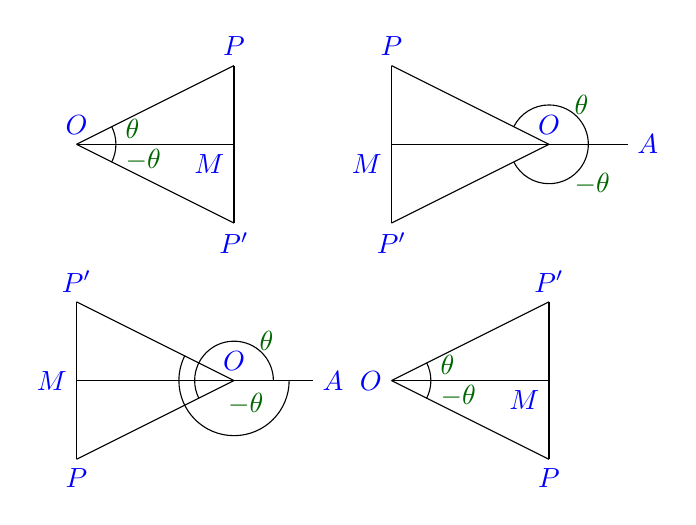
\begin{tikzpicture}
    \draw (0, 0) -- (2, 0);
    \draw (0, 0) -- (2, 1);
    \draw (2, 0) -- (2, 1);
    \draw [blue] (0, 0) node[anchor=south] {$O$};
    \draw [blue] (2, 0) node[anchor=north east] {$M$};
    \draw [blue] (2, 1) node[anchor=south] {$P$};
    \draw [black!60!green] (.5, .2) node[anchor=west] {$\theta$};
    \draw (.5, 0) arc[start angle=0, end angle=27, radius=0.5];
    \draw (0, 0) -- (2, -1);
    \draw (2, 0) -- (2, -1);
    \draw [blue] (2, -1) node[anchor=north] {$P'$};
    \draw (0.5, 0) arc[start angle=360, end angle=333, radius=0.5];
    \draw [black!60!green] (.5, -.2) node[anchor=west] {$-\theta$};

    \draw (6, 0) -- (7, 0);
    \draw (6, 0) -- (4, 0);
    \draw (6, 0) -- (4, 1);
    \draw (4, 0) -- (4, 1);
    \draw [blue] (7, 0) node[anchor=west] {$A$};
    \draw [blue] (6, 0) node[anchor=south] {$O$};
    \draw [blue] (4, 0) node[anchor=north east] {$M$};
    \draw [blue] (4, 1) node[anchor=south] {$P$};
    \draw [black!60!green] (6.2, .5) node[anchor=west] {$\theta$};
    \draw (6.5, 0) arc[start angle=0, end angle=153, radius=0.5];
    \draw (6, 0) -- (4, -1);
    \draw (4, 0) -- (4, -1);
    \draw [blue] (4, -1) node[anchor=north] {$P'$};
    \draw (6.5, 0) arc[start angle=360, end angle=207, radius=0.5];
    \draw [black!60!green] (6.2, -.5) node[anchor=west] {$-\theta$};

    \draw (2, -3) -- (3, -3);
    \draw (2, -3) -- (0, -3);
    \draw (2, -3) -- (0, -2);
    \draw (0, -3) -- (0, -2);
    \draw [blue] (3, -3) node[anchor=west] {$A$};
    \draw [blue] (2, -3) node[anchor=south] {$O$};
    \draw [blue] (0, -3) node[anchor=east] {$M$};
    \draw [blue] (0, -2) node[anchor=south] {$P'$};
    \draw [black!60!green] (2.2, -2.5) node[anchor=west] {$\theta$};
    \draw (2.5, -3) arc[start angle=0, end angle=207, radius=0.5];
    \draw (2, -3) -- (0, -4);
    \draw (0, -3) -- (0, -4);
    \draw [blue] (0, -4) node[anchor=north] {$P$};
    \draw (2.7, -3) arc[start angle=360, end angle=153, radius=0.7];
    \draw [black!60!green] (1.8, -3.3) node[anchor=west] {$-\theta$};

    \draw (4, -3) -- (6, -3);
    \draw (4, -3) -- (6, -2);
    \draw (6, -3) -- (6, -2);
    \draw [blue] (4, -3) node[anchor=east] {$O$};
    \draw [blue] (6, -3) node[anchor=north east] {$M$};
    \draw [blue] (6, -2) node[anchor=south] {$P'$};
    \draw [black!60!green] (4.5, -2.8) node[anchor=west] {$\theta$};
    \draw (4.5, -3) arc[start angle=0, end angle=27, radius=0.5];
    \draw (4, -3) -- (6, -4);
    \draw (6, -3) -- (6, -4);
    \draw [blue] (6, -4) node[anchor=north] {$P$};
    \draw (4.5, -3) arc[start angle=360, end angle=333, radius=0.5];
    \draw [black!60!green] (4.5, -3.2) node[anchor=west] {$-\theta$};
  \end{tikzpicture}
\end{center}

Consider the above diagram which plots the angles of $\theta$ and $-\theta$. Note that $MP$ and $MP'$ are equal in magnitude but
opposite in sign. Thus, we have

$\sin(-\theta) = \frac{MP'}{OP'} = -\frac{MP}{OP} = -\sin\theta$.

$\cos(-\theta) = \frac{OM}{MP'} = \frac{OM}{OP} = \cos\theta$.

$tan(-\theta) = \frac{MP'}{OM} = \frac{-MP}{OM} = -\tan\theta$.

Similarly, $\cot(-\theta) = -\cot\theta, \sec(-\theta) = sec\theta, {\rm cosec}(-\theta) = -{\rm cosec}\theta$.

\section{Angles of $90^\circ + \theta$}
The diagram has been left as an exercise. Similarly, it can be proven that $\sin(90^\circ + \theta) = \cos\theta, \cos(90^\circ +
\theta) = -\sin\theta, \tan(90^\circ + \theta) = -\cot\theta, \cot(90^\circ + \theta) = -\tan\theta, \sec(90^\circ + \theta) =
-{\rm cosec}\theta, {\rm cosec}(90^\circ + \theta) = \sec\theta$.

Angles of $180^\circ + \theta, 270^\circ - \theta, 270^\circ + \theta$ can be found using previous relations.

\section{Angles of $360^\circ + \theta$}
For angles of $\theta$ the radius vector makes an angle of $\theta$ with initial side. For angles of $360^\circ +
\theta$ it will complete a full revolution and then make an angle of $\theta$ with initial side. Thus, the trigonometrical
ratios for an angle of $360^\circ + \theta$ are the same as those for $\theta$.

It is clear that angle will remain $\theta$ for any multiple of $360^\circ$.

\section{Problems}
\begin{enumerate}
\item If $A = 30^\circ,$ verify that
   \begin{enumerate}
   \item $\cos 2A = \cos^2A - \sin^2A = 2\cos^2A - 1$
   \item $\sin 2A = 2\sin A\cos A$
   \item $\cos 3A = 4\cos^3A - 3\cos A$
   \item $\sin 3A = 3\sin A - 4\sin^3A$
   \item $\tan 2A = \dfrac{2\tan A}{1 - \tan^2 A}$
   \end{enumerate}
\item If $A = 45^\circ,$ verify that
  \begin{enumerate}
  \item $\sin 2A = 2\sin A\cos A$
  \item $\cos 2A = 1 - 2\sin^2A$
  \item $\tan 2A = \dfrac{2\tan A}{1 - \tan^2A}$
  \end{enumerate}
\end{enumerate}

Verify that

\begin{enumerate}[resume]
\item $\sin^230^\circ + \sin^245^\circ + \sin^260^\circ = \frac{3}{2}$
\item $\tan^230^\circ + \tan^245^\circ + \tan^260^\circ = 4\frac{1}{3}$
\item $\sin 30^\circ\cos 60^\circ + \sin 60^\circ\cos 30^\circ = 1$
\item $\cos 45^\circ\cos 60^\circ - \sin 45^\circ\sin 60^\circ = -\frac{\sqrt{3} - 1}{2\sqrt{2}}$
\item ${\rm cosec}^245^\circ.\sec^230^\circ.\sin^290^\circ.\cos 60^\circ = 1\frac{1}{3}$
\item $4\cot^245^\circ-\sec^260^\circ + \sin^230^\circ = \frac{1}{4}$
\end{enumerate}

Prove that
\begin{enumerate}[resume]
\item $\sin 420^\circ\cos 390^\circ + \cos(-300^\circ)\sin(-330^\circ) = 1$
\item $\cos 570^\circ\sin 510^\circ -\sin 330^\circ\cos 390^\circ = 0$
\end{enumerate}

What are the values of $\cos A - \sin A$ and $\tan A + \cot A$ when A has the values
\begin{enumerate}[resume]
\item $\frac{\pi}{3}$
\item $\frac{2\pi}{3}$
\item $\frac{5\pi}{4}$
\item $\frac{7\pi}{4}$
\item $\frac{11\pi}{3}$
\end{enumerate}

What values between $0^\circ$ and $360^\circ$ may $A$ have when
\begin{enumerate}[resume]
\item $\sin A = \frac{1}{\sqrt{2}}$
\item $\cos A = -\frac{1}{2}$
\item $\tan A = -1$
\item $\cot A = -\sqrt{3}$
\item $\sec A = -\frac{2}{\sqrt{3}}$
\item ${\rm cosec}A = -2$
\end{enumerate}

Express in terms of the ratios of a positive angle, which is less than $45^\circ,$ the quantities
\begin{enumerate}[resume]
\item $\sin(-65^\circ)$
\item $\cos(-84^\circ)$
\item $\tan 137^\circ$
\item $\sin 168^\circ$
\item $\cos 287^\circ$
\item $\tan(-246^\circ)$
\item $\sin 843^\circ$
\item $\cos(-928^\circ)$
\item $\tan 1145^\circ$
\item $\cos 1410^\circ$
\item $\cot(-1054^\circ)$
\item $\sec 1327^\circ$
\item ${\rm cosec}(-756^\circ)$
\end{enumerate}

What sign has $\sin A + \cos A$ for the following values of $A$?
\begin{enumerate}[resume]
\item $140^\circ$
\item $278^\circ$
\item $-356^\circ$
\item $-1125^\circ$
\end{enumerate}

What sign has $\sin A - \cos A$ for the following values of $A$?
\begin{enumerate}[resume]
\item $215^\circ$
\item $825^\circ$
\item $-634^\circ$
\item $-457^\circ$
\end{enumerate}

\begin{enumerate}[resume]
\item Find the sine and cosine of all angles in the first four quadrants whose tangents are equal to $\cos 135^\circ.$
\end{enumerate}

Prove that
\begin{enumerate}[resume]
\item $\sin(270^\circ + A) = -\cos A$ and $\tan(270^\circ + A) = -\cot A$
\item $\cos(270^\circ - A) = -\sin A$ and $\cot(270^\circ - A) = \tan A$
\item $\cos A + \sin(270^\circ + A) - \sin(270^\circ - A) + \cos(180^\circ + A) = 0$
\item $\sec(270^\circ - A)\sec(90^\circ - A) - \tan(270^\circ - A)\tan(90^\circ + A) + 1 = 0$
\item $\cot A + \tan(180^\circ + A) + \tan(90^\circ + A) + \tan(360^\circ - A) = 0$
\item Find the value of $3\tan^245^\circ - \sin^260^\circ - \frac{1}{2}\cot^230^\circ + \frac{1}{8}\sec^245^\circ$
\item  Simplify $\frac{\sin 300^\circ.\tan 330^\circ.\sec 420^\circ}{\tan 135^\circ.\sin 210^\circ.\sec 315^\circ}$
\item Show that $\tan 1^\circ\tan 2^\circ \ldots \tan 89^\circ = 1$
\item Show that $\sin^25^\circ + \sin^210^\circ + \sin^215^\circ + \ldots + \sin^290^\circ = 9\frac{1}{2}$
\item Find the value of $\cos^2\frac{\pi}{16} + \cos^2\frac{3\pi}{16} + \cos^2\frac{5\pi}{16} + \cos^2\frac{7\pi}{16}$
\end{enumerate}

Find the value of the following:
\begin{enumerate}[resume]
\item $\sec^2\frac{\pi}{6}\sec^2\frac{\pi}{4} + \tan^2\frac{\pi}{3}\sin^2\frac{\pi}{2}$
\item $\cot^230^\circ - 2\cos^260^\circ - \frac{3}{4}\sin^245^\circ - 4\sin^230^\circ$
\item $\frac{\sec 480^\circ{\rm cosec}570^\circ.\tan 330^\circ}{\sin 600^\circ.\cos 660^\circ.\cot 405^\circ}$
\item If $A = 30^\circ,$ show that $\cos^6A + \sin^6A = 1 - \sin^2A\cos^2A$
\item Show that $\left(\tan \frac{\pi}{4} + \cot \frac{\pi}{4} + \sec\frac{\pi}{4}\right)\left(\tan \frac{\pi}{4} + \cot
    \frac{\pi}{4} - \sec \frac{\pi}{4}\right) = {\rm cosec}^2 \frac{\pi}{4}$
\item Show that $\sin^26^\circ + \sin6^212^\circ + \sin^218^\circ + \ldots + \sin^284^\circ + \sin^290^\circ = 8$
\item Show that $\tan 9^\circ.\tan 27^\circ.\tan 45^\circ.\tan 63^\circ.\tan 81^\circ = 1$
\item Show that $\sum_{r = 1}^9 \sin^2\frac{r\pi}{18} = 5$
\item If $4n\alpha = \pi,$ show that $\tan\alpha\tan2\alpha\tan3\alpha. \ldots .\tan(2n - 2)\alpha\tan(2n - 1)\alpha = 1$
\end{enumerate}
